\documentclass[11pt,reqno]{amsart}
\usepackage[T1]{fontenc}
\usepackage{lmodern,amsmath,amssymb,amsthm,mathtools,microtype}
\usepackage[a4paper,margin=28mm]{geometry}
\usepackage{xcolor,tikz,booktabs,enumitem,needspace}
\usetikzlibrary{arrows.meta,positioning}
\definecolor{deepteal}{RGB}{15,81,85}
\usepackage[colorlinks=true,linkcolor=deepteal,citecolor=deepteal,urlcolor=deepteal]{hyperref}
\newtheorem*{theoremA}{Theorem A (Quadratic block repetition)}
\newtheorem*{theoremB}{Theorem B (Interactive noisy communication)}
\newtheorem*{theoremC}{Theorem C (Conditional-comparison reconstruction)}
\providecommand{\tightlist}{\setlength{\itemsep}{0pt}\setlength{\parskip}{0pt}}
\numberwithin{equation}{section}
\setlength{\emergencystretch}{2em}
\setlist[itemize]{leftmargin=*,itemsep=3pt}
\setlist[enumerate]{leftmargin=*,itemsep=3pt}
\hypersetup{pdftitle={Quadratic Repetition for Commuting Projection Games},pdfauthor={Harjas Sandhu},pdfsubject={Conditional reconstruction, parallel repetition and noisy quantum communication}}
\title[Quadratic repetition for commuting games]{Quadratic Repetition for Commuting Projection Games\\and Noisy Quantum Communication}
\author{Harjas Sandhu}
\address{The University of Queensland}
\email{harjas.sandhu@student.uq.edu.au}
\date{7 November 2026}
\subjclass[2020]{Primary 81P45, 46L53; Secondary 68Q17, 94A17}
\keywords{parallel repetition, commuting operators, projection games, conditional relative entropy, quantum correlated sampling, noisy communication}
\begin{document}
\raggedbottom
\begin{abstract}
We prove that a finite two-player Boolean game whose supported winning masks are unions of vertex-disjoint complete bipartite blocks satisfies
\(\omega_{\mathrm{co}}(G^{\otimes n})\le
\exp[-2^{-75}(1-\omega_{\mathrm{co}}(G))^2n]\).
This includes noninjective and partial projection predicates, allows arbitrary within-round question distributions, and holds against arbitrary joint commuting strategies. A separate finite-matrix argument gives the corresponding tensor theorem with its own gap. The quadratic gap power is optimal within the full block class by the known binary line-game lower bound. The main construction gives one exact square-root-weighted conditioned target and two independently normalized one-sided conditional comparisons. Retained-label cancellation, finite-tracial local reconstruction and scalar finite-table closure yield a charged extension and heterogeneous weighted-threshold bounds. We also apply sandwiched-Rényi channel amortization to interactive finite-dimensional protocols: exponential zero-communication soundness survives prescribed memoryless channels below a strict aggregate entanglement-assisted capacity budget. An erasure example has an explicit polynomial-time randomized coding comparator. General quadratic repetition and uniform efficient locality-preserving compilation remain open; no finite-dimensional resource bound is asserted for arbitrary commuting strategies.
\end{abstract}
\maketitle

\section{Introduction}\label{introduction}

Independent tests need not produce independent successes. In a two-player game, each player sees only one part of a question pair and returns an answer without communicating. Even when a referee repeats the experiment with independent questions, the players may use a single joint strategy for the entire string. Parallel repetition asks how quickly the probability of passing every test must fall.

The issue becomes especially delicate for commuting-operator strategies. Here the two players' measurements commute, but they need not act on separate finite-dimensional tensor factors. Finite-dimensional entanglement is a special case. A proof that uses Schmidt decompositions, or approximates a finite tracial algebra by matrices without justification, does not automatically cover this larger model.

We prove a quadratic-gap repetition bound for games whose winning answer graphs are unions of disjoint complete bipartite blocks. This includes projection predicates with noninjective or partially defined maps. The central construction is more general: an exact positive rectangle partition gives one refined conditioned target and two separately normalized one-sided comparison states. Their entropy deficits can be allocated to the untested coordinates. A local reconstruction theorem in finite tracial standard form turns this information bound into legal strategies. Only after eliminating those strategies into scalar inequalities do we pass to arbitrary commuting correlations.

\subsection{Main results}\label{main-results}

A finite Boolean game is a tuple \(G=(X,Y,A,B,\mu,V)\), where all four alphabets are finite and nonempty, \(\mu\) is a probability law on \(X\times Y\), and \(V:X\times Y\times A\times B\to\{0,1\}\). Write \(\omega_{\mathrm{co}}\) for the commuting value and \(\omega_*\) for the supremum over finite-dimensional tensor strategies. A winning mask is \textbf{disjoint-block} if its nonisolated bipartite components are complete bipartite graphs.

\begin{theoremA}
Suppose every supported winning mask of \(G\) is disjoint-block. If
\(\epsilon=1-\omega_{\mathrm{co}}(G)\), then, for every integer \(n\ge1\),
\[
 \omega_{\mathrm{co}}(G^{\otimes n})
       \le \exp(-2^{-75}\epsilon^2n). \tag{A}
\]
The questions may be arbitrarily correlated within each round. The rounds are independent, and the repeated strategy is an arbitrary joint commuting strategy. Separately, the same bound holds for \(\omega_*(G^{\otimes n})\) with its own gap \(\epsilon_*=1-\omega_*(G)\).
\end{theoremA}

No dimension or resource-size bound is asserted. The proof for the tensor gap is carried out in matrices throughout; it is not obtained by substituting \(\epsilon_*\) into a commuting-value inequality. The original binary line games of Kempe and Regev \cite[Definition 3.1 and Theorems 3.2, 4.4]{KR} belong to the full disjoint-block class and show that the power two is optimal there, up to constants. Their endpoint constraints are partial, so this example alone does not settle optimality for total projections.

A second result connects zero-communication soundness with noisy information flow. It uses ordinary finite-dimensional quantum communication; its baseline may be any commuting-value upper bound.

\begin{theoremB}
Let \(H\) be a finite Boolean game and \(q_0=\omega_{\mathrm{co}}(H)\). Suppose finite-dimensional quantum players start with arbitrary shared entanglement independent of the referee questions. They may communicate through a prescribed finite sequence of fixed memoryless channels \(\mathcal N_1,\ldots,\mathcal N_m\), in either direction, with arbitrary local adaptation. Every cross-player signal is included. For every \(\alpha>1\),
\[
 p_{\mathrm{accept}}\le
 \min\left\{1,\exp\left(\frac{\alpha-1}{\alpha}
 [\log q_0+\sum_j I_\alpha(\mathcal N_j)]\right)\right\}. \tag{B}
\]
The reference-marginal-fixed channel information \(I_\alpha\) is defined in (8.1). One common order \(\alpha\) is used for all terms.
\end{theoremB}

Thus an exponential repetition bound can remain exponential in the presence of interactive noisy communication. This statement follows from established replacer-radius and amortization theorems; the contribution is their application at this game interface. We give a source-correlation extension and an explicit erasure-channel example with fully stated coding costs.

\subsection{Predecessors and the precise contribution}\label{predecessors-and-the-precise-contribution}

For unique games, quadratic repetition is already a consequence of the semidefinite-product and rounding machinery of Kempe, Regev and Toner \cite[SDP 3, Lemma 5.7, Theorems 5.2 and 5.5]{KRT}. Commuting strategies supply feasible Gram vectors for that SDP, and its rounding supplies finite tensor strategies. We make no novelty claim for that restriction. Dinur, Steurer and Vidick \cite[Theorem 1, version 2]{DSV} proved exponential repetition for entangled projection games through a multiplicative relaxation; the general gap power in that result is at most twelve, with a stronger linear-gap conclusion for expanding question graphs.

Song's cubic entangled repetition theorem and smooth correlated sampler \cite[Lemma 4.1]{Song}, and Jain's conditional-relative-entropy proof \cite[Definitions 2.6, 2.8; Lemmas 2.24--2.25 and 4.1--4.2]{Jain}, are direct methodological predecessors. We use the copied-question and conditional-comparison framework, but replace finite-dimensional purification arguments by explicit finite-algebra matrices and local polar corrections. The smooth sampler is implemented through tracial graph projections and finite first-success trials; its operational proof is included in Appendix A.

The multivariate trace inequality of Junge and LaRacuente \cite[Theorem I.2 and Lemma VI.2]{JL} supplies the exact-marginal replacement step. Lin's full finite-table closure theorem \cite[Definition 3.1 and Theorem 3.2]{LinTr} then transfers scalar inequalities from finite-tracial strategies to arbitrary commuting strategies. A finite tracial algebra can be infinite dimensional; neither result is a matrix-density statement.

The new construction is the common square-root-weighted target together with two independently normalized one-sided comparisons. They need not be marginals of one common preselection state. Retaining a private copy of the label makes the relevant conditional entropy term cancel exactly. This proves the coordinate reconstruction condition stated as a hypothesis in the earlier entropy-budget paper \cite{Sandhu}. Heterogeneous all-wins and weighted-threshold estimates are consequences of that reconstruction and the scalar allocation argument, rather than separate reconstruction mechanisms.

The communication application uses Gupta and Wilde's replacer-radius identity \cite[Lemma 5]{GW} and Wilde, Berta, Hirche and Kaur's amortization collapse \cite[Proposition 41]{WBHK}. The erasure coding exponent is consistent with the exact strong-converse theorem of Li and Yao \cite[Theorem 6]{LY}; no new channel capacity theorem is claimed.

\section{Conceptual overview}\label{conceptual-overview}

Conditioning on successful tests is powerful and dangerous. It exposes a workspace in which untested answers can look better than any legal one-round strategy. The proof must reconstruct that workspace from a resource chosen before the fresh question arrives. Merely showing that the fresh question law changes little does not suffice.

The argument has five steps. First, resolve the tested winning relation into positive rectangles. Second, coherently record a common rectangle label with amplitude equal to the square root of its weight. Third, compare the resulting single target to two different one-sided positive states. Fourth, allocate the information lost when question references are discarded. Finally, convert small coordinate deficits into one-round strategies. If too many coordinates became too easy at a small conditioning cost, one of those reconstructed strategies would beat the base-game value.

\begin{figure}[ht]
\centering
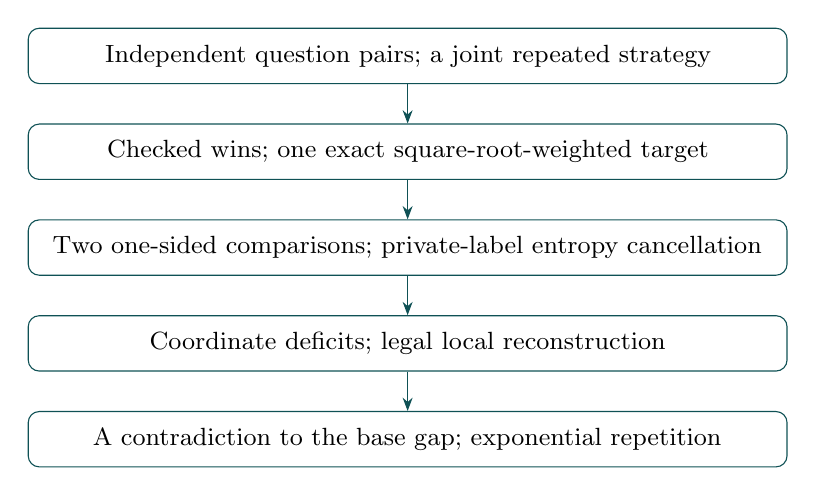
\begin{tikzpicture}[node distance=5mm,
 box/.style={draw=deepteal,rounded corners,align=center,text width=.76\linewidth,inner sep=6pt,font=\small},
 >=Stealth]
\node[box] (a) {Independent question pairs; a joint repeated strategy};
\node[box,below=of a] (b) {Checked wins; one exact square-root-weighted target};
\node[box,below=of b] (c) {Two one-sided comparisons; private-label entropy cancellation};
\node[box,below=of c] (e) {Coordinate deficits; legal local reconstruction};
\node[box,below=of e] (f) {A contradiction to the base gap; exponential repetition};
\foreach \u/\v in {a/b,b/c,c/e,e/f}\draw[->,deepteal] (\u)--(\v);
\end{tikzpicture}
\caption{The proof transfers a conditioned answer table to a legal strategy. It does not interpret postselection itself as a physical protocol.}
\end{figure}

\subsection{A small example: why the weights occur only once}\label{a-small-example-why-the-weights-occur-only-once}

Consider the mask \[
 V=\begin{pmatrix}1&1\\1&0\end{pmatrix}.
\] It has four rectangles of weight \(1/2\): the full first row, the full first column, the singleton upper-right cell and the singleton lower-left cell. Every winning cell is covered with total weight one, while the losing cell is uncovered. The maximum row and column loads are both \(3/2\).

For a fine outcome \((a,b)\), give the common target an orthogonal label \(l\) with coefficient \(\sqrt{w_l}\mathbf1_{R_l}(a)\mathbf1_{T_l}(b)\). The squared norm, summed over labels, is exactly \(V(a,b)\). Both players' original output records can therefore be retained without changing any conditioned measured probability.

Applying two weighted local filters simultaneously would instead multiply the coefficients and produce \(w_l^2\) in the probability. In this example each accepted cell would acquire total weight \(1/2\), not one. The correct construction uses two different comparison states, each of which contains one factor \(\sqrt{w_l}\), against the same target. The comparisons are mathematical witnesses; there is no requirement to apply both filters to a physical resource.

For a disjoint-block mask there is a unique accepted block label, and both load bounds are one. This removes the presentation charge and is exactly where the quadratic gap rate enters. For a general mask the charge can remain positive even when the game gap is small.

\subsection{Two distinctions to keep in view}\label{two-distinctions-to-keep-in-view}

All local measurements produced by reconstruction are complete on every input pair, not only on sampled or synchronized pairs. Sampling failures are charged as actual output branches. And the limiting step concerns finite probability tables: the prepared vectors, algebras and operational witnesses are eliminated before Lin's closure theorem is invoked.

\section{Model and the reusable reconstruction theorem}\label{model-and-the-reusable-reconstruction-theorem}

A commuting strategy uses a unit vector \(\psi\), complete finite POVMs \(P_a^x,Q_b^y\), and \([P_a^x,Q_b^y]=0\) for every input/output pair. Its payoff is \(\sum\mu(x,y)V(x,y,a,b)\langle\psi,P_a^xQ_b^y\psi\rangle\). No optimizer is assumed. In a repeated game each POVM can depend on the entire local question string.

All logarithms are natural. A density is a positive element of trace one; finite classical records use the ordinary sum trace. We use \(\|a\|_p=\tau(|a|^p)^{1/p}\). For bounded densities, \[
 D(\rho\Vert\nu)=\tau\bigl(\rho(\log\rho-\log\nu)\bigr)
\] is the Umegaki relative entropy, with its support-restricted extended-value interpretation. Every difference of divergences below is formed only when both terms are finite. Root fidelity is \(F(\rho,\nu)=\|\sqrt\rho\sqrt\nu\|_1\), and purified distance for normalized states is \(P(\rho,\nu)=\sqrt{1-F(\rho,\nu)^2}\). Data processing means that discarding a register cannot increase relative entropy or purified distance.

First work in finite-tracial standard form: \[
 (\mathcal M,\tau),\qquad
 \mathcal H=L^2(\mathcal M,\tau),\qquad
 \sigma\in\mathcal M_+,\quad\tau(\sigma^2)=1.
\] Alice acts by \(L(a)\xi=a\xi\), Bob by \(R(b)\xi=\xi b\). The right representation is opposite, and commutes with the left representation on every input. The finite von Neumann algebra can be infinite dimensional. Boundedness of \(\sigma\) is part of this starting representation. Subsequent finite amplifications and finite tensor powers preserve that setting.

\subsection{Conditional comparisons}\label{conditional-comparisons}

A question reference is a bookkeeping copy that records how the target depends on the input. It is not a message supplied to a player. Keeping one copy coherent lets us ask whether that dependence can be explained by the original conditional question law and a state prepared on just one side.

The comparison below has exactly that form: its seed contains Alice's local input and workspace, and the factors involving Bob's input come only from the referee's original conditional law. Crucially the seed may have its own local input marginal. Requiring that marginal to agree with the conditioned target would unnecessarily exclude the actual-mass normalization used later.

Let \(\mu\) be a probability law on finite \(X\times Y\), and let \(q\) be supported on its support. Consider bounded unit vectors \(\psi_{xy}\in L^2(\mathcal N)\) in a finite tracial algebra. They determine a copied-input pure family \[
 \sum_{x,y}\sqrt{q(x,y)}
 |x\rangle_{\widehat X}|x\rangle_X
 |y\rangle_{\widehat Y}|y\rangle_Y\psi_{xy}. \tag{3.1}
\] Its Alice marginal is classical in \(\widehat Y\); in each \(y\) block its coherent \(x,x'\) entries are \[
 \sqrt{q(x,y)q(x',y)}\,\psi_{xy}\psi_{x'y}^*.
\] Matching \(\widehat X=X\) copies are understood.

For any positive normalized seed \(T=[T_{xx'}]\) over \(\mathcal N\), an \textbf{Alice conditional comparison} has entries \[
 (\nu_A)_{y;xx'}
 =\sqrt{\mu(y|x)\mu(y|x')}\,T_{xx'}. \tag{3.2}
\] The seed's local \(X\) law is arbitrary on the supported symbols. It need not equal \(q_X\). Bob's comparison is defined by reversing the roles and working over the opposite algebra. These are two separately chosen comparisons for the \textbf{same target}; they need not be margins of a common reference state.

Let \(K_A=XA\), \(K_B=YB\), including all designated residual workspaces. With finite full divergences, define \[
 b_A=D(\rho_A\Vert\nu_A)
       -D(\rho_A^{K_A}\Vert\nu_A^{K_A}),\quad
 b_B=D(\rho_B\Vert\nu_B)
       -D(\rho_B^{K_B}\Vert\nu_B^{K_B}). \tag{3.3}
\] The deficit measures the distinguishability that disappears when the protected question reference is discarded. Data processing makes it nonnegative. A small value says that the reference adds little information beyond the retained local workspace, which is the condition needed for approximate local preparation. The Alice and Bob deficits test different one-sided explanations of the same target.

All quantities are relative-entropy differences of finite displayed values. Infinite individual entropies are not subtracted.

\subsection{Operational reconstruction}\label{operational-reconstruction}

\begin{theoremC}
Under the preceding finite-input, bounded-vector, support, comparison-form, and finite-divergence assumptions, fix finite local/opposite fine POVMs and a Boolean losing predicate. Let \(\alpha\) be its mean loss on the target under \(q\). Put
\[
 t=b_A+b_B+D(q\Vert\mu).
\]
For every \(\zeta>0\), there is one shared resource fixed before the inputs arrive and complete commuting POVMs on \emph{every} local input pair, with loss under \(\mu\) at most
\[
 \boxed{\alpha+K\big(\sqrt\alpha\,t^{1/4}+\sqrt t\big)+\zeta,
 \qquad K=65536.} \tag{3.4}
\]
The resource is a finite amplification and finite tensor power of the original finite algebra. It need not be finite dimensional. The construction preserves the declared fine measurement interface, not an output channel onto the original algebra. Its resource parameters can depend on the entire finite family, spectra, and accuracy; there is no uniform size bound.

\end{theoremC}

The statement does not require a game mask or a repeated-game structure. We prove it next.

\section{Proof of Theorem C}\label{proof-of-theorem-c}

There are three operations. We first replace a conditional comparison by one having exactly the target's retained marginal, while controlling fidelity by the entropy deficit. We then realize the resulting alignment by local polar corrections in a single amplified algebra. Finally, the correlated sampler turns those local descriptions into actual commuting measurements. The losing-event estimate is kept in square-root form so that a nearly perfect target does not pay a generic total-variation error.

\subsection{Exact marginal replacement at positive faithful slack}\label{exact-marginal-replacement-at-positive-faithful-slack}

Write \(r=\rho_K,n=\nu_K\). For Alice, the supported full algebra is \(\bigoplus_{y:\mu_Y(y)>0}M_{X_y}(\mathcal N)\), \(X_y=\{x:\mu(x,y)>0\}\), with the matching fresh-question copies understood; the retained marginal is block diagonal in \(X\). Bob uses the reversed supported corner. Start with boundedly invertible densities there. Set \[
 L_s=r^{(1+is)/2}n^{-(1+is)/2},\qquad
 \widetilde\nu=\int_{\mathbb R}\beta_0(s)L_s\nu L_s^*\,ds,
\quad
 \beta_0(s)=\frac{\pi}{2(\cosh(\pi s)+1)}. \tag{4.1}
\] The integral is normal and all inverse powers are bounded. Its retained marginal is exactly \(r\), since \(L_snL_s^*=r\) pointwise. Because \(K\) is classical in the local question control \(X\), \(L_s\) is \(X\)-block diagonal and commutes with the scalar conditional-amplitude factors in (3.2). Thus \(\widetilde\nu\) remains a conditional comparison. If \(\nu\ge c_\nu I\), \(r\ge c_rI\), and \(n\le M_nI\), then \(\|L_s^{-1}\|\le\sqrt{M_n/c_r}\) uniformly in \(s\), and \(\widetilde\nu\ge(c_\nu c_r/M_n)I\). The following faithful-density arguments therefore apply also to the replacement.

The finite-tracial specialization of Junge--LaRacuente's Theorem I.2 \cite{JL} gives, for positive invertible \(W\), \[
 \tau e^{\log W+\log r-\log n+\log\nu}
 \le\int\beta_0(s)\tau(WL_s\nu L_s^*)\,ds. \tag{4.2}
\] The operator order in this formula is essential. Apply their \(p=2\) inequality to half-logarithms and then scalar Jensen; cyclicity removes the endpoint imaginary powers. This is a primary-source trace-inequality import over general von Neumann algebras, not a matrix-approximation argument.

The Gibbs variational formula and (4.2) imply \[
 b=D(\rho\Vert\nu)-D(r\Vert n)
 \ge \tau(\rho\log W)+1-\tau(\widetilde\nu W).
\] Taking the supremum is the measured-relative-entropy variational formula, hence \[
 D_{\mathrm{meas}}(\rho\Vert\widetilde\nu)\le b,\qquad
 F(\rho,\widetilde\nu)^2\ge e^{-b}. \tag{4.3}
\] Here \(F(a,b)=\|\sqrt a\sqrt b\|_1\) is root fidelity.

The second inequality is valid in finite trace without a dimension assumption. For faithful bounded densities, the positive operator \[
 H=\rho^{-1/2}(\rho^{1/2}\widetilde\nu\rho^{1/2})^{1/2}\rho^{-1/2}
\] satisfies \(H\rho H=\widetilde\nu\). Finite spectral partitions of \(H\) have classical fidelities tending to \(\tau(\rho H)=F\); scalar Jensen gives \(D(p\Vert q)\ge-2\log\sum\sqrt{pq}\). This proves the needed fidelity bound. The measured variational formula follows from operator concavity of \(\log\) in one direction and finite spectral step approximations in the other.

Continuous spectrum at zero requires care. Choose a faithful bounded conditional comparison \(\nu_0\) bounded below on the supported corner, and replace \[
 \rho_\eta=(1-\eta)\rho+\eta\nu_0,\quad
 \nu_\eta=(1-\eta)\nu+\eta\nu_0,\qquad\eta>0. \tag{4.4}
\] Every positive \(\eta\) permits (4.1)--(4.3). The full and retained divergences converge separately to their finite original values. One direct verification uses uniform continuity of \(u\log u\) on a bounded interval, the bound \(\log\nu_\eta\ge\log\nu+\log(1-\eta)\), and a fixed regularizer \(\log(\nu_\eta+\delta I)\) for the reverse limiting inequality. The additional \(\eta\nu_0\log\nu_\eta\) contribution is \(O(\eta|\log\eta|)\). Therefore their difference converges too.

Since \(\rho_\eta\to\rho\) in norm, its square roots converge in \(L^2\), uniformly for comparison with any normalized state. Consequently each positive slack admits an actual normal comparison with \[
 F(\rho,\widetilde\nu_\eta)^2\ge e^{-b}-o_\eta(1). \tag{4.5}
\] There is no claim that inverse powers converge, that removing a kernel creates a spectral gap, or that the comparison states have a normal limiting point. The positive-slack construction suffices.

\subsection{One common amplification and genuinely local corrections}\label{one-common-amplification-and-genuinely-local-corrections}

Let the Alice replacement seed be \(T\in M_k(\mathcal N)\), \(k=|X|\), and write \(C=\sqrt T\), \(r_x=\tau(T_{xx})\). Use unnormalized matrix trace temporarily. In \(\mathcal P=M_k(\mathcal N)\), define \[
 \chi_x=r_x^{-1/2}\sum_z e_{1z}\otimes C_{xz},\qquad
 \psi_{xy}^{\rm emb}=e_{11}\otimes\psi_{xy}. \tag{4.6}
\] The \(\chi_x\) are unit vectors and \(\chi_x\chi_{x'}^*=e_{11}\otimes T_{xx'}/\sqrt{r_xr_{x'}}\). The column index is the finite purifier.

For fixed \(y\), form \[
 A_y=\sum_x e_{x1}\otimes\sqrt{q(x,y)}\psi_{xy},\quad
 B_y=\sum_{xz}e_{xz}\otimes\sqrt{\mu(y|x)}C_{xz}. \tag{4.7}
\] Their left densities are the target and comparison \(y\) blocks. Their fidelity is \(\|A_y^*B_y\|_1\). Polar decomposition supplies \(U_y\) such that \[
 \operatorname{Re}\tau(B_y^*A_yU_y)=\|A_y^*B_y\|_1.
\] It acts by \textbf{right multiplication on purifier columns}, independently of the external coherent \(x\) row. Expanding this trace and applying Cauchy--Schwarz with the normalized comparison law \(r_x\mu(y|x)\) yields \[
 e_A:=\mathbb E_q[1-|\langle\chi_x,\psi_{xy}^{\rm emb}U_y\rangle|^2]
 \le b_A+o(1). \tag{4.8}
\] No equality of the target and comparison \(X\) marginals is used.

The separate Bob comparison bounds the \textbf{same target's} variation: \[
 e_B:=\mathbb E_q P^2(d_{xy},d_y)\le b_B,
\quad d_{xy}=\psi_{xy}^*\psi_{xy},\quad
 d_y=\mathbb E_{x|y}d_{xy}. \tag{4.9}
\] To see the information step, discard the protected copied question in the full divergence, use the conditional comparison form, and subtract the retained divergence. The remaining expression contains \(I(X:B|Y)\) plus a nonnegative question-law divergence. Then use \(P^2\le D\) in natural units. These finite-classical-record identities do not involve infinite entropies.

Write \(\chi_x=J_xu_x\), \(u_x=|\chi_x|\), and set \[
 v_y=[U_y^*(e_{11}\otimes d_y)U_y]^{1/2}.
\] For normalized densities \(a,b\), Hölder with exponents \(4,2,4\) gives \[
 F(a,b)\le[\tau(\sqrt a\sqrt b)]^{1/2},\quad
 \|\sqrt a-\sqrt b\|_2^2\le2P(a,b)^2.
\] Contract (4.8) to the right marginals and use (4.9) and the squared triangle inequality: \[
 \mathbb E_q\|u_x-v_y\|_2^2\le4(b_A+b_B)+o(1). \tag{4.10}
\]

All finite families fit in one finite amplification. Partial polar factors have unitary completions after finite padding; an explicit completion for a partial isometry \(v\) is \[
 \begin{pmatrix}v&I-vv^*\\I-v^*v&-v^*\end{pmatrix}.
\] Left and right completions can use separate finite factors. The corrected fine effects are \[
 A'_x=J_x^*(I\otimes A_x)J_x,\qquad
 B'_y=U_y^*(I\otimes B_y)U_y. \tag{4.11}
\] They are complete POVMs; support-only versions put the complement into a default output. Trace cyclicity checks the Bob orientation. Every left effect commutes with every right effect on all input pairs. Normalizing the matrix trace rescales all vectors by the same square-root factor, leaving probabilities and estimates unchanged.

\subsection{Actual sampling, rare loss, and the fresh law}\label{actual-sampling-rare-loss-and-the-fresh-law}

Apply the standard-form sampler of Appendix A to the finite families \(u_x,v_y\) and the transported fine POVMs. Its contract gives actual unconditional POVMs and, for the \textbf{same protocol}, a losing-event bound \[
 \beta_q\le\alpha'+2\sqrt{\alpha'F_0}+F_0.
\] The rare-event estimate in Appendix A gives \(F_0\le896(h^2+\overline D/h^2)+o(1)\), with \(\overline D\le2D_{\rm desc}+o(1)\). For small positive descriptor discrepancy choose \(h=D_{\rm desc}^{1/4}\); at zero discrepancy take positive \(h\downarrow0\), with inner accuracies chosen first at each \(h\). Equations (4.8)--(4.10) then give, with \(s=b_A+b_B\), \[
 \sqrt{\beta_q}\le\sqrt\alpha+75s^{1/4}+o(1). \tag{4.12}
\] This uses the sampler's actual good-vector and bad-branch estimates. A mean-TV sampler alone would not justify it.

For its all-input losing function \(f(x,y)\in[0,1]\), \[
 |\sqrt{\mathbb E_qf}-\sqrt{\mathbb E_\mu f}|
 \le\|\sqrt q-\sqrt\mu\|_2\le\sqrt{D(q\Vert\mu)}. \tag{4.13}
\] For \(t\le1\), (4.12)--(4.13) imply \[
 \beta_\mu\le\alpha+152\sqrt\alpha\,t^{1/4}
                         +5776\sqrt t+o(1).
\] The remaining regimes use the trivial upper bound one. Both coefficients are below \(65536\). Inner accuracies are taken to zero at a fixed finite family and fixed positive event probability. Every requested positive slack has actual complete POVMs and a fixed resource. This proves Theorem C.

The operational sampler used here is proved in Appendix A. Its first-success selection takes place in an amplified algebra, and its rare-event estimate applies to the actual unconditional output.

\section{The central construction: one target, two one-sided parents}\label{the-central-construction-one-target-two-one-sided-parents}

\subsection{Exact presentation and charge}\label{exact-presentation-and-charge}

For every supported question pair of coordinate \(i\), choose an exact positive fractional rectangle partition \[
 V_i(x,y,a,b)=\sum_lw_{i,xy,l}
                 {\bf1}_{R_{i,xy,l}}(a){\bf1}_{T_{i,xy,l}}(b),
 \quad w_{i,xy,l}\ge0. \tag{5.1}
\] Equality includes losing cells. Let \(A_i(x,y),B_i(x,y)\ge1\) bound its maximum row and column loads, and put \[
 a_i=\mathbb E_{\mu_i}A_i,\quad b_i=\mathbb E_{\mu_i}B_i,\quad
 \kappa_i=\tfrac12\log(a_ib_i). \tag{5.2}
\] The parameter depends on the chosen presentation. Every finite Boolean mask has such a partition, for example singleton winning cells. Disjoint-block masks have unit loads and zero charge. A projection mask is disjoint-block by grouping rows with the same projected output; injectivity is unnecessary.

Consider an arbitrary finite-tracial joint strategy for an independent product of possibly different games. For a proper tested set \(D\), let \(p=\Pr(E_D)>0\), \(L=\log(1/p)\), and \[
 \alpha_i(D)=\Pr\{\text{loss at }i\mid E_D\}.
 \tag{5.3}
\] Fix tested questions \(c=(x_D,y_D)\). Product partitions give one exact mask with weights \(w_{c,l}\) and local load bounds \(A_c=\prod_D A_j(c_j)\), \(B_c=\prod_D B_j(c_j)\).

\subsection{One pure target with the original complete measured table}\label{one-pure-target-with-the-original-complete-measured-table}

Coherently dilate the original full local measurements and retain every fine output on its own side. For live strings \(x,y\) and full fine outputs \(a,b\), write their residual standard-form vector as \(\sqrt{P_a^{c_A,x}}\sigma\sqrt{Q_b^{c_B,y}}\). Append three copies of a common label \(l\) on each target side and use amplitudes \[
 \sqrt{\frac{\mu_J(x,y)w_{c,l}}{p_c}}\,
 {\bf1}_{R_{c,l}}(a_D){\bf1}_{T_{c,l}}(b_D)
 \sqrt{P_a^{c_A,x}}\sigma\sqrt{Q_b^{c_B,y}}. \tag{5.4}
\] Here \(p_c=\Pr(E_D\mid c)>0\). Orthogonality of all fine-output and label registers plus (5.1) gives norm one and \textbf{exactly} the original conditional fine table.

This is a specified mathematical pure target. It is not claimed to arise from a new physically local filter on the original resource. Coherences outside the declared measured table can change. The same target must be used for both comparisons.

One own-label copy stays private in each residual workspace. External copies form the duplicated shared histories, with all such external copies omitted from each comparison parent. Fixing a label leaves a pure target; retaining a cross-created external copy in a reference would invalidate locality and is not done.

\subsection{Separate one-sided parents and positive operator-matrix domination}\label{separate-one-sided-parents-and-positive-operator-matrix-domination}

Alice's one-sided successful coefficients are \[
 \sqrt{w_{c,l}/A_c}\,
 {\bf1}_{R_{c,l}}(a_D)\sqrt{P_a^{c_A,x}}.
\] Their adjoint-products sum to at most identity. Adding the local coefficient \[
 \left[I-\frac1{A_c}\sum_a
       \Big(\sum_lw_{c,l}{\bf1}_{R_{c,l}}(a_D)\Big)P_a^{c_A,x}\right]^{1/2}
\] with a distinct failure sentinel completes a local isometry. Copying the sentinel into the external as well as private label records dephases success/failure when the external records are discarded. Bob has a \textbf{different} completion using \(B_c\) and \(T_{c,l}\). The two completions are not simultaneously applied. This prevents the erroneous coefficient \(w_l^2\).

There is a simpler normalization. Use each uncompleted positive one-sided seed and divide by its actual trace \(G_{A,c}\) or \(G_{B,c}\). Any normalized positive local seed is allowed by (3.2); its question marginal can differ from the target's. Thus no physical reference-preparation claim is required.

For the exact type-II check, at fixed \(y,l\) set \[
 Z_{x,a}=\sqrt{\mu_J(x,y)w_{c,l}}\,
          {\bf1}_{R_{c,l}}(a_D)\sqrt{P_a^{c_A,x}}\sigma .
\] The raw Alice parent is \(S_l=[Z_{x,a}Z_{x',a'}^*]\). The selected target parent is \[
 T_l=[Z_{x,a}Q_{y,T_l}Z_{x',a'}^*],
 \quad Q_{y,T_l}=\sum_{b:b_D\in T_{c,l}}Q_b^{c_B,y}\le I.
\] Therefore \(S_l-T_l\ge0\) by an operator-matrix congruence. No undefined partial trace over an infinite commutant or exchange of same-algebra factors occurs. Bob's calculation is in the opposite algebra.

These comparisons have the original conditional-question form: replace \(\sqrt{\mu_J(x,y)}\) in the Alice seed by \(\sqrt{\mu_{X,J}(x)}\), then attach the scalar conditional factors \(\sqrt{\mu_J(y|x)\mu_J(y|x')}\). Consequently \[
 p_c\rho_{A,c}\le G_{A,c}\nu_{A,c},\qquad
 p_c\rho_{B,c}\le G_{B,c}\nu_{B,c}, \tag{5.5}
\] with \(p_c\le G_{A,c}\le A_c\), \(p_c\le G_{B,c}\le B_c\).

The local-description proof in Section 4 needs one target and two conditional comparisons. It uses Alice's comparison for coherent alignment and Bob's for the same target's marginal variation. It never requires a common reference purification. This is the reason that separate comparison parents suffice.

\subsection{Exact entropy cancellation, tilted averaging, and allocation}\label{exact-entropy-cancellation-tilted-averaging-and-allocation}

For an ensemble \(\rho=\sum_lq_l\rho_l\), Donald's identity on both marginals gives \[
 \begin{split}
 \sum_lq_l[D(\rho_l\Vert\nu)-D(\rho_l^K\Vert\nu^K)]
 &=D(\rho\Vert\nu)-D(\rho^K\Vert\nu^K)
       +I(l:R|K).
 \end{split} \tag{5.6}
\] The private orthogonal label in \(K\) determines \(l\), so the last term is zero, including for question-correlated labels. Order domination in (5.5) then bounds the parent deficit by \(\log(G_{A,c}/p_c)\) or \(\log(G_{B,c}/p_c)\).

Let \(Q_C(c)=\mu_D(c)p_c/p\), \(G_A=\mathbb E_{\mu_D}G_{A,c}\), and similarly \(G_B\). The exact change-of-measure identity is \[
 \mathbb E_{Q_C}\log(G_{A,c}/p_c)
 =L+\log G_A
       -D\!\left(Q_C\middle\Vert
                  \frac{\mu_D(c)G_{A,c}}{G_A}\right)
 \le L+\log G_A. \tag{5.7}
\] Zero-\(p_c\) branches have zero target weight. This is not an exchange of prior and posterior expectations. Product load bounds give \[
 G_A\le\prod_{j\in D}a_j,\qquad
 G_B\le\prod_{j\in D}b_j. \tag{5.8}
\]

For completeness we spell out the ordered allocation, using the copied-register chain rule \cite[Lemma 2.24]{Jain}. Write \(R_i=\widehat X_i\widehat Y_i\). On Alice's side trace \(R_{>i}\), condition only on the classical exposed records \((\widehat Y_{<i},X_{>i})\), and retain the fixed records. Direct-sum relative entropy makes the expected coordinate deficit \[
 D(\rho^{R_{\le i}K}\Vert\nu^{R_{\le i}K})
 -D(\rho^{R_{<i}K}\Vert\nu^{R_{<i}K}).
\] Summing telescopes to the parent deficit. The restriction commutes with attaching the fresh \(i\)-th conditional-question amplitudes, so its comparison form is preserved. Bob uses the reverse order. Both target families are partitions of (5.4): their external histories carry the same \(c,l,Y_{<i},X_{>i}\), their residual spaces carry the complementary coherent questions and the original fine records.

Crucially the local-preparation theorem is applied to the \textbf{whole} \(x_i,y_i\)-indexed target with histories inside its output workspace. The history is not sampled independently beforehand.

The unconditional fresh question marginals \(q_i^{X_iY_i}\) satisfy \[
 \sum_{i\notin D}d_i
 :=\sum_{i\notin D}D(q_i^{X_iY_i}\Vert\mu_i)\le L. \tag{5.9}
\] Indeed event conditioning has density at most \(1/p\) relative to the full product referee law; classical relative entropy to a product dominates the sum of its coordinate marginal divergences.

Set \(t_i=b_{A,i}+b_{B,i}+d_i\). Equations (5.6)--(5.9) and Theorem C prove \[
 \boxed{\sum_{i\notin D}t_i
 \le3L+\log(G_AG_B)
 \le3L+2\sum_{j\in D}\kappa_j,} \tag{5.10}
\] with, for every positive accuracy, legal single-game witnesses of loss \[
 \alpha_i(D)+K\big(\sqrt{\alpha_i(D)}\,t_i^{1/4}+\sqrt{t_i}\big)
       +\text{accuracy}. \tag{5.11}
\] This proves the charged finite-tracial \(\mathrm{FR}(65536)\) condition at the stated exact fractional-partition scope.

\subsection{The parity challenge and why the question quantifier matters}\label{the-parity-challenge-and-why-the-question-quantifier-matters}

Let \(X_i=Y_i\) be iid uniform bits and a sure common checked label be the parity of all live bits. The history \((l,Y_{<i},X_{>i})\) fixes the fresh bit, so \(\sum_i\mathbb E_{\rm history}D(q_i^{XY|\rm history}\Vert\mu_i)=m\log2\) despite \(p=1\). Charging this conditional divergence by \(L=0\) would be false.

Our \(d_i\) is unconditional and equals zero. Histories stay in the full target; both local kernels can generate the same parity from the equal fresh bit and pre-shared outside bits. Equivalently, \[
 D(Q_i^{RXY}\Vert\mu_i Q_i^{R|X})
 =d_i+I(Y:R|X)\le d_i+b_{A,i},
\] and symmetrically for Bob. No conditional-history law is silently replaced by \(\mu_i\). The standalone whole-workspace preparation makes a separate history race unnecessary.

\section{Scalar closure and amplification consequences}\label{scalar-closure-and-amplification-consequences}

\subsection{Eliminate the representation before Lin}\label{eliminate-the-representation-before-lin}

For \(K\ge1\), define \[
 \Phi_K(e,a)=
 \left[\frac{\sqrt{a+4(e-a)_+/K}-\sqrt a}{2}\right]^4. \tag{6.1}
\] Every legal extracted base strategy has loss at least \(\epsilon_i=1-\omega_{\mathrm{co}}(G_i)\). Let the positive accuracy in (5.11) decrease to zero and solve the quadratic in \(t_i^{1/4}\). Equations (5.10)--(5.11) imply \[
 \sum_{i\notin D}\Phi_K(\epsilon_i,\alpha_i(D))
 \le3\log(1/p_D)+\log(G_A(P,D)G_B(P,D)). \tag{6.2}
\]

The actual masses are finite positive linear table functionals. Explicitly, \[
 G_{A,c}(P)=\sum_lw_{c,l}
 \sum_{x_J}\mu_{X,J}(x_J)
 \sum_{a:a_D\in R_{c,l}}P_A(a\mid c_A,x_J), \tag{6.3}
\] and Bob is symmetric. These functionals are independent of the chosen finite-tracial representation. For each tested question \(c\), \(G_{A,c},G_{B,c}\ge p_c\); their prior-averaged masses \(G_A,G_B\) satisfy \(G_A,G_B\ge p_D>0\). It is these averaged masses that occur in (6.2).

Lin's Definition 3.1 and Theorem 3.2 \cite{LinTr} gives full finite-table closure of finite-tracial strategies in \(C_{qc}\). At a fixed \(D\) with target \(p_D>0\), the probabilities, conditional losses, and masses in (6.2) converge. The arguments of the logarithms stay bounded away from zero and \(\Phi_K\) is continuous. Thus (6.2) passes to arbitrary commuting strategies. No raw costs, vectors, algebras, or POVMs are asserted to converge. Finite tracial does not mean finite matrix.

Using (5.8) gives the scalar budget with \(3L+2\sum_D\kappa_j\). This closure is independent of the old resolvent/history proof. It still depends on the exact standalone sampler and Lin's theorem.

\subsection{Quadratic repetition and charged games}\label{quadratic-repetition-and-charged-games}

For an identical block game, (5.10) has zero presentation charge. Here is a complete all-finite-length proof of (A). First suppose a finite-tracial repeated strategy has all-wins probability \(\theta>\exp(-\gamma\epsilon^2n)\), \(\gamma=2^{-75}\), and put \(L_\theta=\log(1/\theta)\). Greedily test a coordinate whose conditional loss exceeds \(\epsilon/2\) while the remaining mean loss does so. Each addition raises log inverse event probability by more than \(\epsilon/2\), while every tested event contains all wins. Fewer than \(2L_\theta/\epsilon<n/2\) coordinates can be tested. At stopping, \(m\ge n/2\), \(p_D\ge\theta\), and mean remaining loss \(\alpha\le\epsilon/2\).

Mix the single-coordinate witnesses with a pre-shared uniform index. Cauchy--Schwarz and Jensen bound its loss by \(\alpha+K[\sqrt\alpha(\mathbb Et_i)^{1/4}+\sqrt{\mathbb Et_i}]\) at arbitrary positive slack. Now \(\mathbb Et_i\le3L_\theta/m<6\gamma\epsilon^2\). Its limiting loss divided by \(\epsilon\) is at most \[
 \frac12+\frac K{\sqrt2}(6\gamma)^{1/4}
                 +K\sqrt{6\gamma}<0.665<1.
\] A sufficiently small finite slack contradicts the base commuting gap. Zero gap or zero all-wins probability is trivial. We have therefore proved a uniform scalar all-wins bound for every finite-tracial table. Applying Lin's finite-table closure to that bound, and only then taking the arbitrary-commuting supremum, proves (A). No operational witnesses or raw \(t_i\) are passed through that limit.

For a common charge \(\kappa\), set \(t_0=1/(256K^4)=2^{-72}\). A live coordinate with conditional loss at most \(\epsilon/2\) has inverse deficit at least \(t_0\epsilon^2\). For this argument, test any live coordinate with conditional loss greater than \(\epsilon/2\) until none remains; do not stop merely when the mean is small. If \(L_\theta=\log(1/\theta)\), the tested set has size at most \(2L_\theta/\epsilon\) and total charge at most \(2\kappa L_\theta/\epsilon\). If the process stops with live coordinates, the scalar budget implies \[
 t_0\epsilon^2(n-2L_\theta/\epsilon)
       \le(3+4\kappa/\epsilon)L_\theta,
\] and hence \[
 L_\theta\ge
 \frac{t_0\epsilon^2n}{3+4\kappa/\epsilon+2t_0\epsilon}
 \ge\frac{2^{-75}\epsilon^3n}{\epsilon+\kappa}.
\] If all coordinates are exhausted, their tested losses already give \(L_\theta\ge n\epsilon/2\), which is stronger. Thus \[
 \boxed{\omega_{\mathrm{co}}(G^{\otimes n})
 \le\exp[-2^{-75}\epsilon^3n/(\epsilon+\kappa)].} \tag{6.4}
\] For zero gap the exponent is interpreted as zero, including when \(\kappa=0\). For general masks, singleton rectangles give a general cubic-gap estimate. A row-star partition has one unit load and the other at most \(|A|\); a column-star partition reverses the roles. Hence one may always take \[
 \kappa\le\tfrac12\log\min\{|A|,|B|\}. \tag{6.5}
\] This refinement follows by choosing the smaller of the row-star and column-star presentations.

\textbf{The gap power is optimal within the full block class.} The original binary line game \(L_m\) of Kempe--Regev has only equality masks and endpoint singleton masks, all of which are disjoint-block. Definition 3.1 and Theorem 3.2 of \cite{KR} give matching classical and no-signalling values, so \[
 1-\omega_{\mathrm{co}}(L_m)=\epsilon_m=\frac1{2m-1}.
\] Theorem 4.4 of \cite{KR} gives a classical repeated lower bound \((1-O(m^{-2}))^n\) for \(n\ge m^2\). Thus an absolute constant \(C\) satisfies \[
 \omega_{\mathrm{co}}(L_m^{\otimes n})
 \ge\omega(L_m^{\otimes n})
 \ge \exp[-C\epsilon_m^2n]\qquad(n\ge m^2)
\] for all sufficiently large \(m\). A universal exponent \(f(\epsilon)\) with \(f(\epsilon_m)/\epsilon_m^2\to\infty\) would contradict this lower bound. The power two in (A) is therefore optimal for its full disjoint-block class, up to constants. This does not optimize \(2^{-75}\), establish priority, or show optimality for the narrower class of total projections: the endpoint predicates in this fixture are partial.

For the tensor statement, start with a finite tensor strategy and use a full matrix standard form. Every step above, including all sampler copies, stays a full finite matrix algebra; its left/right action is a genuine finite tensor resource. The greedy contradiction therefore uses \(\epsilon_*\), uniformly before the supremum. This does not assert equality of tensor and commuting values.

\subsection{Heterogeneous games and weighted thresholds}\label{heterogeneous-games-and-weighted-thresholds}

Let \(\epsilon_i=1-\omega_{\mathrm{co}}(G_i)\), assume \(\kappa_i\le C_0\epsilon_i\), and put \[
 S=\sum_i\epsilon_i^2,\qquad
 Z=\sum_i\epsilon_i{\bf1}\{\text{loss at }i\}.
\] The following consequences hold: \[
 \boxed{\omega_{\mathrm{co}}(\bigotimes_iG_i)
 \le\exp[-2^{-75}S/(1+C_0)],} \tag{6.6}
\] \[
 \boxed{\Pr\{Z\le(1-r)S\}
 \le\exp[-2^{-85}r^5 S/(1+C_0)],
 \quad0<r\le1.} \tag{6.7}
\] For blocks \(C_0=0\). The zero-\(S\) interpretation is the trivial upper bound one.

For clarity, the scalar deduction of (6.7) is included. Set \(M_D=3\log(1/p_D)+2\sum_D\kappa_i\). Apply the inverse deficit (6.1), cap the conditional loss by \(\alpha_i'=\min(\alpha_i,\epsilon_i)\), and use Hölder to obtain \[
 S_D-A_D\le K[S_D^{3/4}M_D^{1/4}+\sqrt{S_DM_D}],
\quad S_D=\sum_{i\notin D}\epsilon_i^2,\ 
 A_D=\sum_{i\notin D}\epsilon_i\alpha_i(D).
\] The cap is necessary for the Hölder step.

Independently include \(i\) in a random tested set with probability \(u\epsilon_i/(1+u\epsilon_i)\), and condition its selected tests to succeed. Its normalization is \[
 F(u)=\mathbb E\prod_i(1+u\epsilon_i)^{-{\bf1}\{\text{loss at }i\}},
\quad L(u)=-\log F(u).
\] The posterior entropy identity gives \(\mathbb E\log(1/p_D)\le L(u)\), while \(\mathbb ES_D\ge(1-u)S\) and \(\mathbb E\sum_D\kappa_i\le C_0uS\). Under the tilted outcome law \(T_u\), \[
 \mathbb E_{T_u}Z\ge(1-u)S
 -K[S^{3/4}\overline M^{1/4}+\sqrt{S\overline M}],
\quad\overline M\le3L(u)+2C_0uS,
\] \[
 L'(u)\ge\mathbb E_{T_u}Z/(1+u).
\] Take \(\lambda=r^4/[2^{20}K^4(1+C_0)]\). Wherever \(0\le u\le\lambda\) and \(L(u)\le\lambda S\), the error is below \(rS/16\); thus \(L'(u)\ge(1-r/4)S\). By monotonicity, either \(L(\lambda)\ge\lambda S\) or this derivative bound integrates throughout the interval. In both cases \(L(\lambda)\ge(1-r/4)\lambda S\). On \(Z\le(1-r)S\) the product defining \(F(\lambda)\) is at least \(e^{-\lambda(1-r)S}\). Therefore the event probability is at most \(e^{-r\lambda S/2}\), which is (6.7) for \(K=2^{16}\). Full tested sets contribute zero live mass; zero-probability tested events have zero posterior weight.

For (6.6), test a positive-gap coordinate whenever its conditional loss exceeds \(\epsilon_i/2\). Then \(\sum_D\epsilon_i\le2L_\theta\), \(\sum_D\epsilon_i^2\le2L_\theta\), and \(\sum_D\kappa_i\le2C_0L_\theta\). With \(t_0=1/(256K^4)=2^{-72}\), a conditional loss at most \(\epsilon_i/2\) forces \(\Phi_K\ge t_0\epsilon_i^2\). Hence \(t_0(S-2L_\theta)\le(3+4C_0)L_\theta\), which implies (6.6). Exhausting every positive-gap coordinate gives the bound directly.

The intrinsic rate \(\exp[-c\sum_i\epsilon_i^3/(\epsilon_i+\kappa_i)]\) without a bounded ratio is still open. One must not multiply bounds for separate groups.

\section{Finite resources and the operational interface}\label{finite-resources-and-the-operational-interface}

The reconstruction theorem supplies a legal strategy at each positive accuracy. It does not supply a uniform implementation cost. Its finite matrix amplifications add ordinary finite ancillary records; finite tensor powers permit independent first-success trials. The original finite von Neumann algebra remains present. When it is infinite dimensional, the resulting strategy need not have a finite matrix realization.

This distinction is also needed in an abelian algebra. Let \(\mathcal M=\mathbb C^2\), with equal trace weights, and let the two possible target vectors be \(\sqrt2e_0\) and \(\sqrt2e_1\). An algebra-local trace-preserving channel with Kraus coefficients in \(\mathcal M\) fixes every central projection in the adjoint picture: \[
 \sum_j K_j^*zK_j=z\sum_jK_j^*K_j=z.
\] It cannot move the fixed central weights of one resource to either requested sector. This rules out a stronger output-channel interpretation of reconstruction.

Finite first-success selection avoids that obstruction. Independent copies of the tracial resource contain independent central samples. When the players request the same sector, their local success predicates agree on every trial. After \(N\) trials their common failure probability is \(2^{-N}\), and the chosen copy is in the requested sector. The resulting output probabilities arise from complete POVMs on the amplified resource. On nonsynchronized branches there is no promised state in the original algebra.

More generally, if the finite spectral approximations in Appendix A have largest positive singular value \(B_0\) and smallest \(\delta_0\), the label count and trial count can be chosen with \[
 l\le\left\lceil\frac{\log(B_0/\delta_0)}h\right\rceil+4,\qquad
 S\le\frac{e^{2h}B_0^2}{1-e^{-2h}},\qquad
 N=\left\lceil e^{2h}S\log(2/\xi)\right\rceil .
\] The error constant is uniform, but these resources need not be. No efficient acquisition of spectral data for an arbitrary von Neumann algebra is assumed.

Consequently the finite-table closure used in Section 6 is applied to scalar probabilities only. It neither preserves the constructed descriptors nor gives a finite-dimensional approximation to an arbitrary commuting strategy. The separate tensor theorem avoids this issue by beginning in matrices and remaining there.

\section{Interactive noisy-channel verification: proof and exact scope}\label{interactive-noisy-channel-verification-proof-and-exact-scope}

For finite density matrices, use the sandwiched divergence \[
 D_\alpha(\rho\Vert\sigma)
 =\frac1{\alpha-1}\log\operatorname{Tr}
 [(\sigma^{(1-\alpha)/(2\alpha)}\rho
                 \sigma^{(1-\alpha)/(2\alpha)})^\alpha].
\] Inverse powers are restricted to the comparison support; the divergence is \(+\infty\) when \(\operatorname{supp}\rho\not\subseteq\operatorname{supp}\sigma\). Trace distance below means \(\tfrac12\|\rho-\sigma\|_1\). Define \[
 I_\alpha(\mathcal N)
 =\sup_{\psi_{RQ}\ {\rm pure}}\inf_{\zeta_B}
 D_\alpha(({\rm id}_R\otimes\mathcal N)(\psi)
                         \Vert\psi_R\otimes\zeta_B). \tag{8.1}
\] The unchanged-reference marginal is fixed. Some simulation papers reverse this orientation; that alternative is not substituted.

\subsection{Complete proof of Theorem B}\label{complete-proof-of-theorem-b}

The initial shared state is independent of the full referee question record and the laboratories initially receive only their respective local questions. Section 8.2 handles correlated initial resources with an additional source cost.

Gupta--Wilde \cite[Lemma 5, (5.16), (5.19)--(5.20)]{GW} gives \[
 I_\alpha(\mathcal N)=\inf_\zeta
 D_\alpha(\mathcal N\Vert\mathcal R_\zeta),\quad
 \mathcal R_\zeta(Z)=\operatorname{Tr}(Z)\zeta.
\] Wilde--Berta--Hirche--Kaur \cite[Proposition 41, (283)]{WBHK} gives, for arbitrary different input states and arbitrary reference memories, \[
 D_\alpha(\mathcal N(\rho_{RQ})\Vert\sigma_R\otimes\zeta)
 \le D_\alpha(\rho_{RQ}\Vert\sigma_{RQ})
                  +D_\alpha(\mathcal N\Vert\mathcal R_\zeta).
 \tag{8.2}
\] This amortization collapse is for a channel versus a replacer, not for two arbitrary channels.

Choose almost-minimizing replacers separately for each prescribed slot and fixed \(\alpha\). Compare the real interactive protocol with the same local protocol in which every cross-player channel is replaced by its fixed local discard-and-prepare map. Include all referee questions, outputs, memories, and both laboratories in the reference for (8.2). Initially the states agree. Between slots, the same local maps cannot increase divergence. At slot \(j\), (8.2) adds at most \(I_\alpha(\mathcal N_j)\) plus arbitrarily small slack. The final divergence is at most their sum, regardless of local feedback or transmission direction.

The all-replacer experiment is a legal zero-communication quantum strategy with acceptance \(q\le q_0\). Apply the same binary acceptance measurement to both final states. Binary data processing gives \[
 D_\alpha(\operatorname{Ber}(p)\Vert\operatorname{Ber}(q))
 \ge\frac{\alpha}{\alpha-1}\log p-\log q.
\] This proves (B), after removing finite slack. If \(q_0=0\), finite channel costs force \(p=0\); if \(q_0=1\), cap at one. The argument supplies no unrestricted infinite-algebra Rényi statement about communicating arbitrary-co resources.

\subsection{Source correlations, smoothing, and transcript errors}\label{source-correlations-smoothing-and-transcript-errors}

Let the actual normalized cq initial state be \(\rho_{UAB}\), where \(U\) is the full referee question record and \(A,B\) are the device resources before ordinary local question copies are delivered. For one question-independent resource \(\sigma_{AB}\), suppose \[
 J_\alpha\ge D_\alpha(\rho_{UAB}\Vert
        \sum_u\mu_H(u)|u\rangle\langle u|\otimes\sigma_{AB}).
\] The same telescope yields \[
 p\le\inf_{\alpha>1}\exp\!\left\{
 \frac{\alpha-1}{\alpha}
 [\log q_0+J_\alpha+\sum_jI_\alpha(\mathcal N_j)]\right\}. \tag{8.3}
\] Every term must use the \textbf{same} order. A normalized cq state within trace distance \(\eta\) of a state satisfying the displayed Rényi bound adds \(\eta\) once, after the whole protocol.

There is a different algebraic source interface. If the complete controlled acceptance effects obey \[
 P_{\rm actual}\le e^hP_{\rm independent}+\eta
\] by a certified hockey-stick/order defect, then the valid finite-order consequence is \[
 p\le\eta+e^h
 \inf_{\alpha>1}
 e^{\frac{\alpha-1}{\alpha}(\log q_0+\sum_jI_\alpha(\mathcal N_j))}. \tag{8.4}
\] This interface yields (8.4); moving \(h\) inside the Rényi factor is not justified by the normalized-smoothing argument. For example \(\rho=|0\rangle\langle0|\), \(\sigma=|+\rangle\langle+|\), multiplier two, has hockey-stick defect \((\sqrt5-1)/2\), but its nearest normalized state dominated by \(2\sigma\) is at trace distance \(1/\sqrt2\). These two smoothing notions are not equivalent. This example distinguishes the interfaces; it does not rule out every stronger inequality under additional assumptions.

If the referee tolerates a nonnegative integer \(r\) failed coordinates and an adversary can edit a nonnegative integer \(t\) coordinate answer records after the interaction and after seeing the transcript, while the referee retains its original questions, acceptance implies at most \(r+t\) original failures. Apply (B) or (8.3) to that original threshold event. For a threshold with \(\delta=\epsilon-(r+t)/n>0\), one may apply any available general-game threshold bound. The block bound below is proved here. For identical blocks use (6.7), with \(r_{\rm rel}=\delta/\epsilon\), giving the available rate \(2^{-85}\delta^5/\epsilon^3\). An actual perfect honest strategy remains accepted under \(t\) edits when the tolerance is at least \(t\); supremum-one completeness is preserved as a supremum. No noisy honest implementation is assumed.

\subsection{Capacity-rate consequence and exact channel assumptions}\label{capacity-rate-consequence-and-exact-channel-assumptions}

Suppose \(\omega_{\mathrm{co}}(H_n)\le e^{-gn}\). Channels come from a fixed finite family \(\mathcal M_l\), with prescribed slot counts \(m_l(n)/n\to\beta_l<\infty\), in any prescribed order/directions. Their environments are independent and inaccessible; no timing, routing, identity-selection, or classical control signal is free.

Finite-dimensional continuity \(I_\alpha\to C_E\) at order one implies exponential soundness if \[
 \sum_l\beta_lC_E(\mathcal M_l)<g. \tag{8.5}
\] Choose one fixed order sufficiently close to one with a strict margin and apply (B). For arbitrary \(n\)-dependent correlated sources, a bound on \(J_1/n\) alone is insufficient; require a fixed-order margin in (8.3), or a justified uniform/iid Rényi-regularity condition.

Noiseless classical \(c\)-bit and quantum \(q\)-qubit channels have costs \(c\log2\) and \(2q\log2\) at every order. Letting \(\alpha\to\infty\) recovers the factors \(2^c,4^q\). The noiseless factors also follow from transcript guessing and teleportation. Our finite-order theorem is stated for finite-dimensional protocols; it is not an assertion about arbitrary normal communicating maps on von Neumann algebras.

For arbitrary finite channels a direct maximum-order comparison uses \[
 M(\mathcal N)=\min\{\operatorname{Tr}S:
              S\ge0,\ I_Q\otimes S\ge J_{\mathcal N}\}.
\] Here \(J_{\mathcal N}=\sum_{r,s}|r\rangle\langle s|\otimes\mathcal N(|r\rangle\langle s|)\) is the unnormalized Choi matrix. CP order gives \(p\le q_0\prod_jM(\mathcal N_j)\), reference-uniformly. This is the known channel max-information/simulation quantity, not a new invariant.

\section{Concrete strict gain and matched coding comparator}\label{concrete-strict-gain-and-matched-coding-comparator}

For a \(d\)-dimensional erasure channel with survival \(s\), \[
 \mathcal E_{s,d}(\rho)=s\rho\oplus(1-s)\operatorname{Tr}(\rho)|e\rangle\langle e|,
\] the exact costs are, with \(u=(\alpha-1)/\alpha\), \[
 I_\alpha(\mathcal E_{s,d})
 =u^{-1}\log[1-s+s d^{2u}],\quad
 C_E=2s\log d,\quad I_\infty=\log(1-s+sd^2). \tag{9.1}
\] To verify the formula, compare to \(zI_d/d\oplus(1-z)|e\rangle\langle e|\). A pure input's successful-block power is bounded using its at most \(d\) Schmidt coefficients, with equality for a maximally entangled input. Twirling that input shows arbitrary replacers cannot improve it. Minimizing \(a^\alpha z^{1-\alpha}+b^\alpha(1-z)^{1-\alpha}\), \(a=sd^{2u},b=1-s\), gives \((a+b)^\alpha\). Thus both sides match. The same value at maximum order follows from CP domination of the erasure and surviving blocks.

There is a strict transfer for every certified exponent \(0<g\le1/4\). Allow one qubit-erasure slot per game coordinate with \(s=3g/(8\log2)\). Order \(\alpha=4/3\) gives \[
 p_n\le e^{-gn/64}, \tag{9.2}
\] while both raw qubit counting and the optimum per-slot maximum-order cost are vacuous. Indeed \(I_{4/3}<15g/16\), whereas \(\log(1+3s)>g\). This includes the conservative exponents of the present repetition results. For tiny \(g\) the required erasure rate is correspondingly extreme; no practical efficiency follows.

A completely solvable comparator makes the gain concrete. Let Alice receive a uniform \(n\)-bit string, Bob receive one fixed question, and require Bob to output that string. Its commuting zero-communication value is exactly \(2^{-n}\). Allow \(4n\) forward qubit-erasure slots with survival \(1/10\). Counting charges \(4\log4>\log2\); exact maximum-order domination charges \(4\log(13/10)>\log2\). Both fail. The finite-order bound gives \[
 p_n\le e^{-E_*n},\qquad
 E_*=4D_{\rm bin}(1/8\Vert1/10)
      =0.01297370627\ldots>1/100. \tag{9.3}
\] The maximizing \(u\) satisfies \(4^u=9/7\).

For even \(n\), an explicit randomized linear protocol achieves \[
 \frac9{32(4n+1)}e^{-E_*n}
 \le p_{\rm construction}\le p_{\rm optimal}\le e^{-E_*n}. \tag{9.4}
\] Pre-share \(4n\) EPR pairs and a uniform binary \(8n\times n\) matrix \(B\). Alice dense-codes consecutive pairs of \(BX\) into the EPR halves and sends them through the slots. Bob reads surviving pairs and samples uniformly from the affine solution space. With \(K=n/2\) surviving slots, the resulting square random binary matrix is invertible with probability at least \(9/32\). The binomial type probability is at least \((4n+1)^{-1}e^{-4nD_{\rm bin}(1/8\Vert1/10)}\). Multiplication proves (9.4).

Costs: \(4n\) transmitted qubits, \(4n\) EPR pairs, \(8n^2\) pre-shared random bits, \(O(n^2)\) encoding work and \(O(n^3)\) binary elimination work. There is no exponential codebook or unreported deterministic-code acquisition. The described decoder is a finite binary-elimination algorithm. The resource analysis assumes ideal dense coding and the specified memoryless erasures.

The exact channel-coding exponent agrees with Li--Yao \cite[Theorem 6]{LY}. This construction is a matched demonstration of the theorem's strength, not a new coding theorem.

\section{Limitations and further questions}\label{limitations-and-further-questions}

The reconstruction theorem and its block-game consequence have different scopes. Exact positive fractional rectangle partitions exist for all finite Boolean predicates, so the charged scalar inequality is general. Quadratic repetition follows when the presentation charge vanishes, or more generally when it is controlled by the gap. The proof does not show that a general predicate admits such a presentation. A state-sensitive entropy allocation that avoids the positive-presentation charge remains the decisive missing operation for arbitrary-predicate quadratic repetition.

The weighted threshold estimate has a fifth-power deviation rate. The present argument does not identify that power as optimal. Likewise, the heterogeneous intrinsic exponent \[
 \sum_i\frac{\epsilon_i^3}{\epsilon_i+\kappa_i}
\] is not proved without a uniform charge-to-gap bound. Bounds for separate groups cannot simply be multiplied, since the repeated strategy may correlate their outputs.

Two elementary counterexamples delimit the communication and reconstruction interfaces. First, reveal a uniform \(n\)-bit string completely with probability \(1/n\), and reveal nothing otherwise. Expected communication is one bit, and the mutual information is \(\log2\), but the guessing probability is at least \(1/n\). Expected communication or Shannon leakage alone cannot preserve an exponential soundness guarantee. The finite-order conditions in Section 8 carry indispensable tail information.

Second, take independent uniform bits \(X,Y,A,B\) and condition on \(A\oplus B=XY\). The event has probability \(1/2\) for every input, so the question law is unchanged. Nevertheless the conditioned box wins CHSH perfectly, whereas its commuting value is at most \((2+\sqrt2)/4\). Small question drift alone therefore does not legalize postselection. Our reconstruction pays both preparation deficits and the unconditional question-law cost.

Finally, repetition is not a locality-preserving Hamiltonian construction. It does not by itself provide bounded local consistency tests, an acquired finite encoding, a controlled energy normalization or an efficient honest implementation. Nor does it supply uniform polynomial-size certificates for cryptographic compilation of a growing family of games. These require additional constructive theorems. The noisy-channel application is an information-theoretic statement for its stated protocol model, rather than an implemented device advantage.

\section*{Acknowledgements and AI use}

The mathematical ideas, constructions, proofs, and manuscript were developed by GPT-6 Astra, with additional AI assistance for review. Human input was minimal and consisted primarily of setting the research objectives and providing occasional feedback.

\appendix

\section{Operational tracial correlated sampling}\label{operational-tracial-correlated-sampling}

We give the sampler needed in Section 4, including its losing-event estimate. Smooth logarithmic labels and first-success sampling are adapted from Song \cite[Lemma 4.1]{Song}. The finite-tracial implementation below uses graph projections and keeps all output branches.

Let \((\mathcal M,\tau)\) be finite with faithful normal tracial state. Let \(a_x,b_y\) be finite families of unit \(L^2(\mathcal M,\tau)\) vectors, and let \(A_x^s,B_y^t\) be complete finite POVMs in \(\mathcal M\), represented on the left and right, respectively. For a law \(\nu\), put \[
 D=\mathbb E_\nu\|a_x-b_y\|_2^2,\qquad
 p_{xy}(s,t)=\langle a_x,L(A_x^s)R(B_y^t)a_x\rangle .
\] The sampler supplies one input-independent resource in a finite amplification and tensor power, and complete all-input commuting POVMs. More precisely, for \(0<h<1/2\), bounded finite-spectrum approximations of accuracy \(\eta>0\), and timeout parameter \(\xi>0\), its actual loss obeys \[
 \beta\le\alpha+2\sqrt{\alpha F}+F,\qquad
 F=896\left(h^2+\frac{2D+8\eta^2}{h^2}\right)+3\eta^2+\xi ,
 \tag{A.1}
\] where \(\alpha\) is the loss of the declared target table and the losing effect may depend arbitrarily on \(x,y\). All approximation and timeout parameters are chosen before the realized questions.

\subsection{Spectral coupling and finite approximations}\label{spectral-coupling-and-finite-approximations}

For spectral decompositions \(c=\sum_i\lambda_iE_i\), \(d=\sum_j\mu_jF_j\), tracial orthogonality gives \[
 \left\|\sum_{ij}z_{ij}E_iF_j\right\|_2^2
       =\sum_{ij}|z_{ij}|^2\tau(E_iF_j).
 \tag{A.2}
\] Indeed left orthogonality removes unequal \(i\), and trace cyclicity removes unequal \(j\). The coefficients \(\tau(E_iF_j)\) are nonnegative and have the correct spectral marginals. Applying this coupling to self-adjoint dilations \[
 Z_a=\begin{pmatrix}0&a\\a^*&0\end{pmatrix}
\] and the scalar \(1\)-Lipschitz map \(t\mapsto|t|\) gives \[
 \||a^*|-|b^*|\|_2^2\le2\|a-b\|_2^2. \tag{A.3}
\] No commutation of \(a,b\) is required.

Approximate each vector by a bounded element, normalize, take its polar decomposition and approximate its positive left modulus by a finite spectral step function. The interval nearest zero may be set to zero. Normalizing again gives unit approximations \(\bar a_x,\bar b_y\), of error at most \(\eta\), with finite-spectrum left moduli. Since the input families are finite, all choices can be made together. Their mean discrepancy satisfies \[
 \bar D\le2D+8\eta^2. \tag{A.4}
\]

\subsection{Smooth labels and graph projections}\label{smooth-labels-and-graph-projections}

For \(\lambda>0\), set \(s=-\log\lambda/h\), \(k=\lfloor s\rfloor\), \(t=s-k\), and \[
 g_\lambda=\cos(\pi t/2)|k\rangle+\sin(\pi t/2)|k+1\rangle.
\] Use one finite integer interval covering every positive spectral value of the approximating family, and add an orthogonal label \(o\). Negative integers are allowed. Set \[
 T=\sum_k e^{-kh}e_{kk}\otimes1,\quad T|o\rangle=0,\quad
 S=(\operatorname{Tr}_l\otimes\tau)(T^2),\quad
 \Omega=T/\sqrt S .
\] The label space and \(\Omega\) depend on the finite family, not on the realized input. Direct scalar estimates give \[
 \|(T-\lambda)g_\lambda\|\le2h\lambda,\qquad
 \lambda\mu(1-|\langle g_\lambda,g_\mu\rangle|^2)
       \le\pi^2(\lambda-\mu)^2/h^2, \tag{A.5}
\] and \[
 \mu|1-\langle g_\lambda,g_\mu\rangle|
       \le\pi|\lambda-\mu|/h.
\] For the latter estimates use the speed \(\pi/2\) of the label curve when the logarithmic separation is at most \(h\); otherwise use the trivial overlap bound and \(|\lambda-\mu|\ge\max(\lambda,\mu)h/2\). Zero coefficients have zero multiplier and are omitted from the following graph maps.

For a fixed approximating pair \(a,b\), put \(c=|a^*|\), \(d=|b^*|\), \(b=du\). Define in \(\mathcal K=M_l\otimes\mathcal M\) \[
 F_c=\sum_k e_{ko}\otimes g_k(c),\quad P_c=F_cF_c^*,\qquad
 F_d=\sum_k e_{ko}\otimes g_k(d),\quad P_d=F_dF_d^*.
\] Here \(g_k(0)=0\). These are graph partial isometries and projections. Alice's success coefficient is \(K_A=F_c^*\); Bob's is \(K_B=F_d(e_{oo}\otimes u)\). Thus \[
 K_A^*K_A=P_c,\qquad K_BK_B^*=P_d.
\] The reversed Bob order is essential because \(R(v)R(w)=R(wv)\).

Write, using the unnormalized matrix trace, \[
 A=\|P_cT\|_2^2,\quad B=\|TP_d\|_2^2,\quad
 C=\|P_cTP_d\|_2^2,\quad U=A+B-C.
\] Their normalized values are the local success, joint success and union probabilities. Trace cyclicity gives the exact identity \[
 m=A+B-2C=\|P_cT-TP_d\|_2^2,\qquad
 U\ge\max(A,B)\ge e^{-2h}. \tag{A.6}
\] If \(\Delta=\|a-b\|_2^2\) and \(r=h^2+\Delta/h^2\), then (A.2)--(A.5) give \[
 m\le128r,\qquad
 K_ATK_B=e_{oo}\otimes x,\qquad
 \|x-b\|_2^2\le40r. \tag{A.7}
\] For clarity, the two spectral calculations behind these constants are \[
 \|F_ccF_c^*-F_ddF_d^*\|_2^2
 =\sum_{ij}\bigl[(\lambda_i-\mu_j)^2+
 2\lambda_i\mu_j(1-|\langle g_{\lambda_i},g_{\mu_j}\rangle|^2)\bigr]
 \tau(E_iF_j)
\] and \[
 x=\sum_{ij}\langle g_{\lambda_i},Tg_{\mu_j}\rangle E_iF_ju.
\] Each of \(\|P_cT-F_ccF_c^*\|_2^2\) and \(\|TP_d-F_ddF_d^*\|_2^2\) is at most \(4h^2\). The three-term squared triangle inequality and (A.3) give \(m\le24h^2+6\Delta+12\pi^2\Delta/h^2\le128r\). For the second calculation the coefficient error is at most \(8h^2\mu_j^2+2\pi^2(\lambda_i-\mu_j)^2/h^2\), giving \(\|x-b\|_2^2\le8h^2+4\pi^2\Delta/h^2\le40r\). If \(C>0\), the normalized vector \(v=x/\sqrt C\) satisfies \(\|v-b\|_2\le2\sqrt{40r}\). Its conditional output uses the original fine POVMs after local label erasure.

\subsection{Complete finite first-success protocol}\label{complete-finite-first-success-protocol}

Use \(N=\lceil e^{2h}S\log(2/\xi)\rceil\) independent copies of \(\Omega\). Each player keeps its first local success, with a fixed default answer on timeout. Alice's underlying effects are \[
 E_x^s=\sum_{j=1}^N(1-P_c)^{\otimes(j-1)}
 \otimes[K_A^*(I_l\otimes A_x^s)K_A]\otimes1^{\otimes(N-j)}
 +\mathbf1_{s=s_0}(1-P_c)^{\otimes N}.
\] Bob's underlying effects are \[
 F_y^t=\sum_{j=1}^N(1-P_d)^{\otimes(j-1)}
 \otimes[K_B(I_l\otimes B_y^t)K_B^*]\otimes1^{\otimes(N-j)}
 +\mathbf1_{t=t_0}(1-P_d)^{\otimes N}.
\] They are positive and sum to identity by telescoping. The physical effects are \(L_N(E_x^s)\) and \(R_N(F_y^t)\). They commute for every pair of inputs, even when the retained trial indices differ.

Independence of trials gives the exact probability of a common retained index: \[
 w_{\mathrm{same}}=\frac C U[1-(1-U/S)^N],\qquad
 1-w_{\mathrm{same}}\le e^{2h}m+\xi\le384r+\xi. \tag{A.8}
\] On that branch the output is the table on \(v\). Every other branch is a genuine output branch and is charged loss at most one.

For the original target \(a_x\), the approximation and (A.7) give \[
 \|v-a_x\|_2^2\le512r_{xy}+3\eta^2 .
\] For a positive losing effect \(0\le M_{xy}\le I\), the triangle inequality for \(M_{xy}^{1/2}\) gives its synchronized loss at most \((\sqrt{\alpha_{xy}}+\sqrt{512r_{xy}+3\eta^2})^2\). Combining with (A.8), and then Cauchy--Schwarz in the average, proves (A.1). If \(C=0\), the entire branch is charged, and the same upper bound holds. This proof controls a rare losing event for the actual unconditional POVMs, not merely a mean total-variation distance.

All approximations, label ranges and trial counts are finite at fixed positive parameters. One first chooses \(h>0\), then sufficiently small \(\eta,\xi\). At zero discrepancy one takes positive \(h\) tending to zero with those inner errors. No inverse spectral gap, zero-width label or infinite-time protocol is used.

\section{Register placement and entropy allocation}\label{register-placement-and-entropy-allocation}

We record the register assignment behind Section 5. This makes clear why the two comparison states concern the same target and why the shared history need not be sampled independently.

Fix tested questions \(c\) and a successful label \(l\). Keep three copies of the label on each target side. Each residual workspace \(E_A,E_B\) retains its own private copy and all its original fine outputs. Partition the other four copies as \[
 H_{A,\mathrm{label}}=(L_A^1,L_B^3),\qquad
 H_{B,\mathrm{label}}=(L_B^1,L_A^3).
\] They contain identical values on the accepted target. All four external copies are omitted from the comparison parents; otherwise a Bob-created label in Alice's reference could destroy its conditional form.

For live \(i\), the histories and residual bodies are \[
\begin{aligned}
 H_{A,i}&=(c,H_{A,\mathrm{label}},\widehat Y_{<i},X_{>i}),&
 A_i^0&=\widehat X_{<i}X_{<i}E_A,\\
 H_{B,i}&=(c,H_{B,\mathrm{label}},Y_{<i},\widehat X_{>i}),&
 B_i^0&=\widehat Y_{>i}Y_{>i}E_B .
\end{aligned}
\] Together with \(\widehat X_i,X_i,\widehat Y_i,Y_i\), these partition one pure vector. Redundant equal history copies can be suppressed by fixed isometries. The original coordinate answer is read from its local retained fine-output record.

The ordered restrictions on Alice's comparison trace the later protected references and expose only \((Y_{<i},X_{>i})\); Bob uses the reverse orientation. These restrictions act outside the fresh protected reference and hence commute with attaching its original conditional-question amplitudes. For each orientation the relative-entropy increments telescope: \[
 \sum_i\bigl[D(\rho^{R_{\le i}K}\Vert\nu^{R_{\le i}K})
             -D(\rho^{R_{<i}K}\Vert\nu^{R_{<i}K})\bigr]
 =D(\rho^{RK}\Vert\nu^{RK})-D(\rho^K\Vert\nu^K).
\] Direct-sum relative entropy identifies each exposed classical branch with the corresponding expected coordinate deficit. This is the ordered copied-reference identity of Jain \cite[Lemma 2.24]{Jain}; no finite-dimensional entropy subtraction is required, since all displayed relative entropies are finite by domination. The private label in \(K\) makes its additional conditional mutual information zero.

Finally, apply reconstruction to the whole \(x_i,y_i\)-indexed pure target, with the histories included in its output workspace. They are not first sampled from a posterior law. The separately charged question divergence is the unconditional \(D(q_i\Vert\mu_i)\). In particular, conditioning a history that reveals the fresh question does not create an uncharged external source.

Finite target ancillas can all be embedded in one common standard form. For \(\psi=\sum_{ab}|a\rangle|b\rangle w_{ab}\), map it to \[
 \sqrt{d_Ad_B}\sum_{ab} e_{a1}\otimes e_{1b}\otimes w_{ab}
 \ \in L^2(M_{d_A}\otimes M_{d_B}\otimes\mathcal M),
\] with normalized matrix traces. Alice's matrix acts on the left first factor and Bob's transposed matrix on the right second factor. For operator-valued Bob matrices the transpose accompanies the opposite coefficient algebra; this is the canonical opposite-algebra isomorphism, not a positive-partial-transpose assumption. Thus every assignment above has exact all-input left/right locality.

\begin{thebibliography}{99}
\bibitem{Sandhu} H. Sandhu.
Entropy Budgets and Weighted Concentration in Parallel Games.
Preprint, 2026.
\href{https://doi.org/10.5281/zenodo.23987561}{doi:10.5281/zenodo.23987561}.
\bibitem{KRT} J. Kempe, O. Regev and B. Toner.
Unique games with entangled provers are easy.
\emph{SIAM J. Comput.} \textbf{39}(7), 3207--3229 (2010).
Version used: \href{https://arxiv.org/abs/0710.0655v3}{arXiv:0710.0655v3}.
\bibitem{KR} J. Kempe and O. Regev.
No strong parallel repetition with entangled and non-signaling provers.
\href{https://arxiv.org/abs/0911.0201v1}{arXiv:0911.0201v1} (2009).
\bibitem{DSV} I. Dinur, D. Steurer and T. Vidick.
A parallel repetition theorem for entangled projection games.
\emph{Comput. Complexity} \textbf{24}, 201--254 (2015).
Version used: \href{https://arxiv.org/abs/1310.4113v2}{arXiv:1310.4113v2}.
\bibitem{Song} Z. Song.
Parallel repetition for entangled games with gap exponent three.
\emph{Electronic Colloquium on Computational Complexity},
Report TR26-199 (2026).
\url{https://eccc.weizmann.ac.il/report/2026/199/}.
\bibitem{Jain} R. Jain.
Parallel repetition for entangled games via conditional relative entropy.
\href{https://arxiv.org/abs/2610.21410v1}{arXiv:2610.21410v1} (2026).
\bibitem{JL} M. Junge and N. LaRacuente.
Multivariate trace inequalities, \(p\)-fidelity, and universal recovery beyond tracial settings.
\emph{J. Math. Phys.} \textbf{63}, 122204 (2022).
\href{https://doi.org/10.1063/5.0066653}{doi:10.1063/5.0066653}.
Version used: \href{https://arxiv.org/abs/2009.11866v2}{arXiv:2009.11866v2}.
\bibitem{LinTr} J. Lin.
Tracially embeddable strategies: Lifting \(\mathsf{MIP}^*\) tricks to \(\mathsf{MIP}^{\mathrm{co}}\).
\href{https://arxiv.org/abs/2304.01940v3}{arXiv:2304.01940v3} (2025).
\bibitem{GW} M. K. Gupta and M. M. Wilde.
Multiplicativity of completely bounded \(p\)-norms implies a strong converse for entanglement-assisted capacity.
\emph{Commun. Math. Phys.} \textbf{334}, 867--887 (2015).
Version used: \href{https://arxiv.org/abs/1310.7028v3}{arXiv:1310.7028v3}.
\bibitem{WBHK} M. M. Wilde, M. Berta, C. Hirche and E. Kaur.
Amortized channel divergence for asymptotic quantum channel discrimination.
\emph{Lett. Math. Phys.} \textbf{110}, 2277--2336 (2020).
\href{https://doi.org/10.1007/s11005-020-01297-7}{doi:10.1007/s11005-020-01297-7}.
Version used: \href{https://arxiv.org/abs/1808.01498v2}{arXiv:1808.01498v2}.
\bibitem{LY} K. Li and Y. Yao.
Strong converse exponent for entanglement-assisted communication.
\emph{IEEE Trans. Inform. Theory} \textbf{70}(7), 5017--5029 (2024).
\href{https://doi.org/10.1109/TIT.2023.3335219}{doi:10.1109/TIT.2023.3335219}.
Version used: \href{https://arxiv.org/abs/2209.00555v3}{arXiv:2209.00555v3}.
\end{thebibliography}

\end{document}
